\documentclass{chi2009}
\usepackage{times}
\usepackage{url}
\usepackage{graphics}
\usepackage{color}
\usepackage[pdftex]{hyperref}
\usepackage[]{algorithm2e}
\hypersetup{%
pdftitle={Your Title},
pdfauthor={Your Authors},
pdfkeywords={your keywords},
bookmarksnumbered,
pdfstartview={FitH},
colorlinks,
citecolor=black,
filecolor=black,
linkcolor=black,
urlcolor=black,
breaklinks=true,
}
\newcommand{\comment}[1]{}
\definecolor{Orange}{rgb}{1,0.5,0}
\newcommand{\todo}[1]{\textsf{\textbf{\textcolor{Orange}{[[#1]]}}}}

\usepackage{subfig}

\pagenumbering{arabic}  % Arabic page numbers for submission.  Remove this line to eliminate page numbers for the camera ready copy

\begin{document}
% to make various LaTeX processors do the right thing with page size
\special{papersize=8.5in,11in}
\setlength{\paperheight}{11in}
\setlength{\paperwidth}{8.5in}
\setlength{\pdfpageheight}{\paperheight}
\setlength{\pdfpagewidth}{\paperwidth}

% use this command to override the default ACM copyright statement 
% (e.g. for preprints). Remove for camera ready copy.
\toappear{Final project Paper}

\title{A Visualization Tool for Human-in-the-loop Machine Learning}
\numberofauthors{2}
\author{
  \alignauthor Marco Tulio Ribeiro \\
    \affaddr{Computer Science and Engineering}\\
    \affaddr{University of Washington}\\
    %\affaddr{Affiliation}\\
    \email{marcotcr@cs.washington.edu}
  \alignauthor Brian Dolhansky\\
    \affaddr{Computer Science and Engineering}\\
    \affaddr{University of Washington}\\
    \email{bdol@cs.washington.edu}
}

\maketitle

% \begin{abstract}
%   In this paper we describe the formatting requirements for SIGCHI
%   Conference Proceedings, and offer recommendations on writing for the
%   worldwide SIGCHI readership.  Please review this document even if
%   you have submitted to SIGCHI conferences before, for some format
%   details have changed relative to previous years. These include the
%   formatting of table captions, the formatting of references, and a
%   requirement to include ACM DL indexing informati:n.
% \end{abstract}

% \keywords{put author keywords here} 
% 
% \category{H.5.2}{Information Interfaces and Presentation}{Miscellaneous}[Optional sub-category]

%TODO:
%It seems to be a consensus amongst machine learning researchers and
%practitioners that ``we need to spend more time with the data'', ...

\section{Introduction}
As the amount of data produced by the world’s population increases year by year,
the need for efficient ways to process and learn from that data arises. The
field of machine learning, a marriage of statistics and computer science, is one
attempt at distilling large amounts of data into a usable format. However, many
machine learning models are difficult to interpret, or they learn something
different from the true desire of their designers. 

Our project brings a human into the “learning loop” (see Figure \ref{hmloop}) so
that more accurate models can be produced. The idea is that we would start with
a trained machine learning
model (\emph{train} and \emph{model} boxes). The system (or the user) would then
pick a set of examples and/or summary statistics to look at(\emph{pick} box),
which are then explained to the user in some way (\emph{explain box}). Having
understood what the model's strengths and weaknesses, the user is in a position
of providing some sort of feedback (\emph{feedback box}), which could be in the
form of labeling more examples, adding or removing features, changing models,
etc. The loop then starts again. This formulation of the problem encompasses
techniques like active learning (amongst many others), where \emph{pick} is the
most important step, and \emph{feedback} involves labeling examples, while
\emph{explain} is ignored.

\begin{figure}[hb]
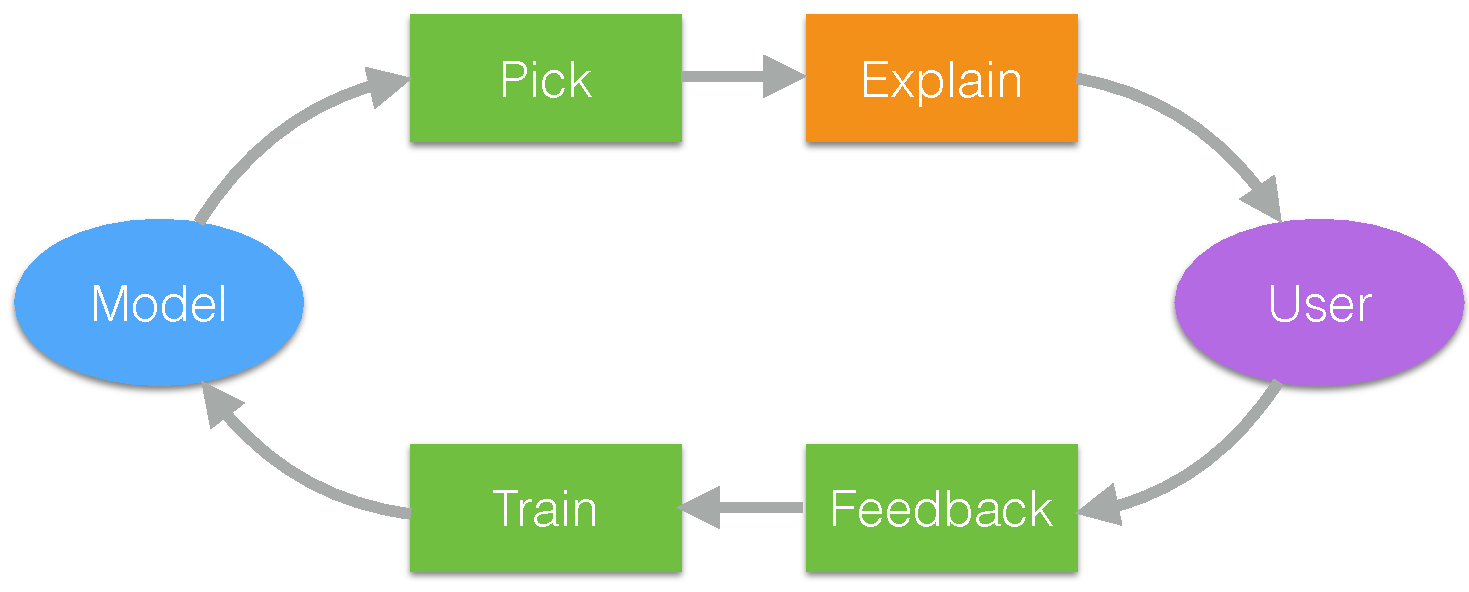
\includegraphics[width=.5\textwidth]{feedback_loop_cropped.pdf}
\caption{Machine learning loop}
\label{hmloop}
\end{figure}

The critical part in the loop where visualization comes is the \emph{explain}
box. This involves giving an overview of what the models are learning, as well
as explaining individual predictions. This is the primary focus of this work -
along with a simple mechanism for \textbf{feedback}, which is required if we are
to have a full loop. We focus primarily on text data, and on the multi-class
classification task. For simplicity, we assume that the bag-of-words
representation is used, although we plan on relaxing this assumption in future
work, as our visualizations generally do not depend on it.

Our tool has three top ``views'', which share a common visualization underneath
that allows the users to interact with the dataset. The first view is meant to explain
individual predictions to users, in terms of feature contributions. The second
view gives the users a global ``summary'' of the model, in the form of summary
statistics and an interactive confusion matrix. Finally, the third view allows
the user to give feedback to the model. The kind of feedback we allow currently
concerns mainly data cleaning - which we argue is already important enough to
significantly improve most text classifiers.


\section{Literature Review}
The statement that understanding what machine learning models are really
learning leads to better models is not very controversial.  Patel et al
\cite{Patel:2008:ISM:1357054.1357160} conducted interviews with machine learning
/ HCI practitioners, and found a consensus regarding the following: (1) the
machine learning process is iterative and exploratory, (2) understanding data
and algorithms is really important, and (3) evaluation is hard and critical.
They do a study where they observe people trying to produce a digit classifier,
where they found that a lot of time people get stuck in part of the process
(e.g. model selection) when the problem is somewhere else (such as lack of
labeled data, or noise in the data). They also found that just looking at
summary statistics in cross validation (CV) data is not enough for evaluation -
all of the participants overestimated their models’ accuracy, when compared to a
hidden test set, due to CV quirks. This led the authors to produce Gestalt
\cite{gestalt}, a system aimed at software developers that exposes the Machine
Learning pipeline in steps. One can see a particular example all the way through
the pipeline, implement his own visualization, click on a confusion table to see
misclassified examples and click on an example and see the features or the raw
data. Unfortunately, no explanation of how the model is interacting with the
data is provided to the user, so it may be hard to determine what to do to
improve the model.

On a similar line of research, \cite{modeltracker} provides a
visualization where examples are sorted according to the model's prediction, and
colored by their true class (which was the inspiration for our databin
visualization). You can click on an example to see the raw data. Any interaction
(adding features, relabeling examples, etc) which makes an example move produces
an arrow from the previous position to the next position. Their visualizations
are helpful, but there is no support for multi-class classification, or
explanation of why the model is making predictions the way it is. Also, the
visualization does not scale to larger datasets, as there is not enough space in
the screen for all of the points.

Some research has been done on explaining individual predictions, or giving an
overall explanation for the model. In \cite{explain:krr15}, the authors
``distill'' a matrix factorization model into rules (trying to be faithful to
the original model, while being more interpretable). It is unclear as to how
helpful these are, as there is still a problem of selecting which rules to show
to the user. In \cite{Strumbelj:2010:EEI:1756006.1756007}, the authors focus on
explaining individual classifications by highlighting individual feature
contributions, taking into account the interactions between features. Contrary
to the name, their method is not efficient at all, as it takes over an hour to
generate an explanation for an individual prediction in a dataset with 279
features (which is very modest for today's standards), so it could not be used
for interactive visualization.

More in line with our vision of machine learning as a loop,
\cite{Stumpf:2009:IMM:1555003.1555106} did an experiment where the system
explained itself to the user by showing rules, Na\"{i}ve Bayes ``weights'' or
similar examples to the one being classified. The users then provided free form
feedback (on paper), which they later tried to incorporate retroactively. Both
their explanations and some of their feedback are model-dependent, working only
with Na\"{i}ve Bayes. In fact, in follow up work
\cite{Kulesza:2011:WED:2030365.2030367} they develop an interactive system
focused only on Na\"{i}ve Bayes, where the explanation is guided by user questions,
such as ``why is this example classified positive''. One drawback of their
system is that feedback is very limited (just relabeling documents), and it's
not clear how useful it is - in fact it seems that it usually harms the
system's performance. It is also not very interactive, which is a feature that
most participants in their study really wanted - being able to change something
and seeing the results right away. 

Our main contributions are combining all of the following in one system: (1)
treating the process as a loop and allowing for feedback, (2) explaining individual
predictions - visually and interactively, (3) allowing for multiclass
classification, (4) interactivity in both the individual prediction explanations
and ``global'' model explanations, (5) handling larger datasets (to a certain
extent), and (6) being model-agnostic - i.e. working with any machine learning
classification model.

\section{The Backend, Feature Importance}
We wrote the backend of our visualization in python, on top of
scikit-learn\footnote{http://scikit-learn.org/}. We used different text dataset
corpora, but in this report we will restrict our examples to subsets of the 20
newsgroups dataset\footnote{http://qwone.com/~jason/20Newsgroups/}. This is a
widely used dataset in the literature, and it consists of distinguishing between
emails sent to different newsgroups. In this report, we either use a 2-class
subset which tries to distinguish between Christianity and Atheism newsgroups,
or a 3-class subset which tries to distinguish between ``windows-misc'',
``ibm-hardware'' and ``windows-x''. As a classification algorithm, all of our
examples use L2 regularized logistic regression, although any classification
algorithms that produces class prediction probabilities can be used in our tool.

In order to assess the importance of a feature (in our case, word) to a
prediction, we follow a greedy procedure. We assume our classifier can return
$P(Y=y|x)$ for any $x$, and that the classifier predicts the example as $y$
(i.e. $pred(x) = y$). If
the example being explained is $x$, we start with $x' = x$ and define $x'_{-w}$
as a copy of $x'$ without feature $w$. We follow the procedure outlined in
Algorithm 1, which removes words from $x$ until the class changes. The
importance of a word is then defined as how much it influences the prediction if
it is re-added to $x$ afterwards.

\begin{algorithm}
 let $x' = x$\;
 let $words = list()$\;
 \While{$pred(x') = y$ and $x'$ is not empty}{
  $w' = {\operatorname{argmax}}_w \quad P(Y=y|x') - P(Y=y | x'_{-w})$\;
  append $w'$ to $words$\;
  \If{$pred(x') \ne y$}{
   Append to $words$ every word $w'$ such that $pred(x'_{-w'}) \ne y$\, and
   remove every such $w'$ from $x'$;
   }
 $x' = x'_{-w'}$\;
 }
 \ForEach{$w \in words$} {
  Importance$(w)$ = $p(Y=y | x'_{-w}) - p(Y=y | x')$;
 }
 \caption{Explain prediction $y$ for example $x$}
\end{algorithm}

Although it is greedy and approximate, this algorithm has the following
advantages: (1) it is relatively fast, assuming fast predictions are available
(which is usually the case), (2) it is general, so that any classifier that
outputs a prediction probability can be explained, and (3) the explanation has
an easy interpretation: if all of the words that are explained as important
were removed, the prediction changes.

\section{The Databin}
\begin{figure}
  \subfloat[Likelihood binning]{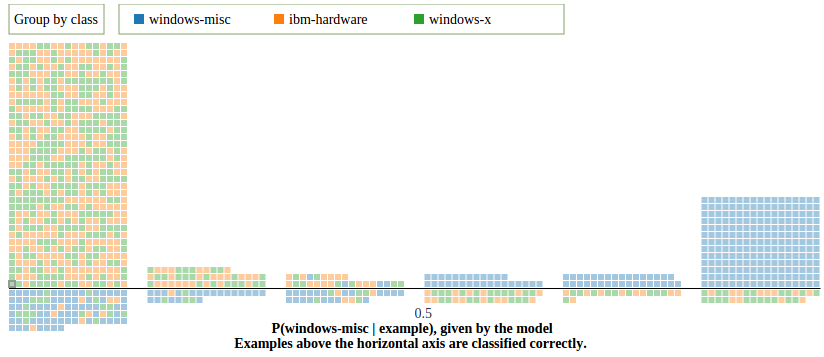
\includegraphics[width=.5\textwidth]{likelihood_bin}}\\
  \subfloat[Class binning]{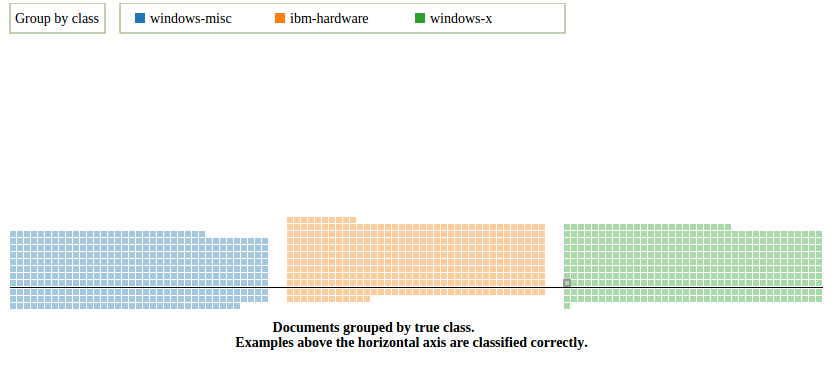
\includegraphics[width=.5\textwidth]{class_bin}}
  \caption{Two databin modes}
  \label{fig:databin}
\end{figure}

The main tool we use for visualizing a dataset as a whole is the
\textit{databin} (see Figure~\ref{fig:databin}). With this visualization, the
user is given an overview of how the model classifies each document. In
addition, the databin is interactive, and allows users to examine certain
documents by clicking on them, or seeing more information about an example by
hovering over it. With the encodings we've chosen, it is immediately evident
what documents the model may be overfitting on, thereby speeding up the Explain
and Feedback steps.

This visualization is similar to and inspired by \cite{modeltracker}, but with
several notable changes. A major limitation of Modeltracker is that it cannot
handle more than two classes, but most non-trivial machine learning
classification problems consist of multiple classes. Hence, we've used different
encodings and interactions in order to represent the performance on multiple
classes in a two-dimensional space. In addition, in contrast to the positional
encodings used by Modeltracker and our initial databin mode (\textit{likelihood
binning}), we've added an additional mode (which we call \textit{class
binning}). In this mode, examples can be binned by class instead of their model
likelihood. 

\textbf{Likelihood binning} In this mode, each example $x_i$ is represented with
a single square whose color is determined by the true class of the example $y_i$
We encode the likelihood $p(y\ |\ x_i)$ of an example $x_i$ belonging to a
particular class $y$ with the horizontal bin of the square. The class $y$
can be changed by clicking on the corresponding legend entry, and any changes
are animated. We use the vertical position to encode whether or not an example
was classified correctly. All examples whose true class $y_i$ equals the model's
prediction $y$ are binned above the horizontal line, and vice versa for
mistakes. This makes it very simple to see which examples the model has
classified incorrectly. For instance, the model is very confident on examples at
either extreme of the horizontal. If there exist some examples below the
horizontal line at these extremes, then the model has made a very confident
mistake, which is usually indicitive of some underlying problem that needs to be
rectified by a user.

\textbf{Class binning} We can use an alternative horizontal encoding to see the
performance on all classes in parallel. Instead of using the likelihood to
encode which bin an example, we simply bin each class separately. We still use
the same vertical and color encodings. In this mode, it is simple to see if a
model is underperforming on one class in particular.

One criticism that could be construed against the databin is that it is limited
to small datasets. In order to minimize this problem, we make the bin sizes
adaptative to the number of documents that would fall in each bin - i.e. if
there are enough documents in a bin to violate the vertical boundaries, we use
less bins. If that is not enough, we reduce the size of the squares encoding the
documents. While these measures still donot allow for huge datasets, it makes the
visualization more flexible to medium-sized datasets.

\section{Explaining individual predictions}
% TODO: Add some anecdotal evidence that this is useful
\section{Global statistics}
\begin{figure}
  \subfloat[Cells in the confusion matrix are
  interactive]{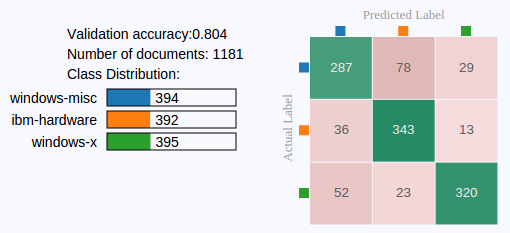
\includegraphics[width=.5\textwidth]{statistics}}\\
  \subfloat[When a cell is clicked, the corresponding examples are
  brushed]{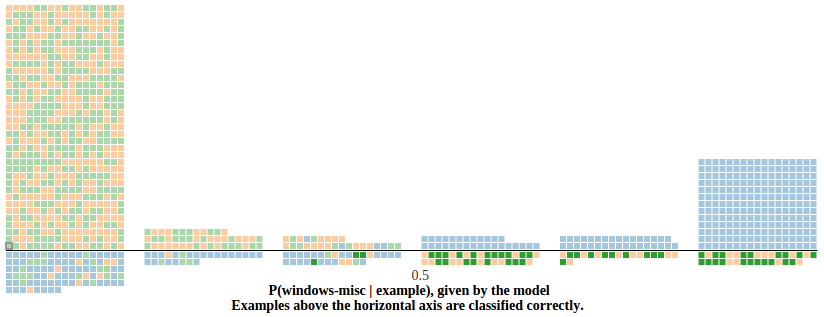
\includegraphics[width=.5\textwidth]{statistics_brush}}
  \caption{The global statistics visualization.}
  \label{fig:statistics}
\end{figure}

If the user wants a more quantitative view of the model performance, they can
select the ``Global Statistics'' tab, which includes standard metrics such as
accuracy and the label distributions. In addition, an interactive confusion
matrix is included. We note here that we got the confusion matrix design from
one of the TAs. The user can select one of the cells in the matrix, and the
corresponding entries are brushed in the databin (see
Figure~\ref{fig:statistics}). This aids the user in determining why a certain
class of mistakes is made, by examining the examples in that class. For
instance, a user may want to figure out if there is a common pattern in the
``windows-misc'' class that the model classifies as ibm-hardware. Doing so
yields the quick observation that the model is not robust to the presence of
``hardware'' words in other classes, such as ``disk'', ``backup'', or even
``computer''. We know that such words would be expected in ``windows-misc'', as
windows runs on hardware. This king of insight allows us to determine what the
next steps should be when trying to improve our classifier.
\section{Feedback}
\begin{figure}
  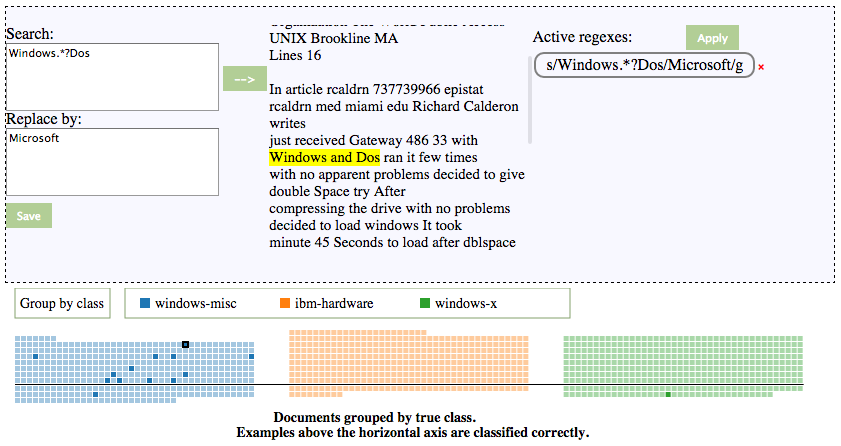
\includegraphics[width=.5\textwidth]{feedback}
  \caption{Data cleaning feedback.}
  \label{fig:feedback}
\end{figure}
In order to close the loop, the user must be able to provide some feedback to
the sytem. In this work, we let the user perform basic data cleaning, in the
form of search and replace regular expressions. As shown in Figure
\ref{fig:feedback}, we highlight the parts of each
document that match the search regular expression, in order to help the user
come up with the correct expression. We also ``brush'' the examples in the
databin that match it, so that the user can gauge the impact of the feedback
before applying it. When a set of regular expressions is applied, it modifies
every example it matches on the training and validation sets, and the classifier
is retrained on the backend. Even this simple form of feedback already has a tremendous
impact - one is able to remove very common words, remove parts of the document
that may lead to overfitting (e.g. headers in the 20 newsgroups dataset), and
etc.
\section{Conclusions / Future work}
In this work, we propose and implement a tool that enables human-in-the-loop
machine learning. We primarily focused on the ``explain'' aspect, which allows
the practitioner to understand what kind of concepts the system is learning, and
why. We also provide a simple form of feedback, which allows for data cleaning.
Since our tool has a lot of features, we built a tutorial using
Trip.js\footnote{http://eragonj.github.io/Trip.js/}, which guides you through
each of the features interactively.
We received a lot of positive feedback when presenting the poster for this work.
Some notable comments were to the effect of ``this is great - I took a machine
learning course last quarter and it really bothered me that I didn't know what
it was learning, or how to improve it'', or ``are you guys thinking of turning
this into a startup?''.

As for future work, an obvious next step is doing a user study to validate the
usefulness of our tool. We claim that our system allows users to come up with
models that generalize better, so a study where models are evaluated on a held
out dataset that was collected in a different manner than the training and
validation datasets seems like the right approach. Another line of work would be
overcoming the databin size limitation, by aggregating nearby points into
``clusters'', which could then be expanded by hovering or clicking. More work on
the feedback side of the picture would greatly improve the usefulness of the
tool. One can imagine the full range of feature engineering being done in the
tool - and maybe even model and hyperparameter selection. Someone in the poster
session suggested that we allow for explanations of classes other than the
predicted one - so that one could know how to ``force'' the model to predict the
right class, and not only to stop predicting the wrong one. Finally, one last
line of work would be to expand this to other kinds of data, such as images and
tabular data, which are widely used in the scientific community.


\bibliographystyle{abbrv}
\bibliography{sample}

\end{document}
